\documentclass[11pt]{article}
\usepackage{euscript}
\usepackage{amsmath}
\usepackage{amsthm}
\usepackage{amssymb}
\usepackage{epsfig}
\usepackage{xspace}
\usepackage{amsmath,amssymb,amsthm}
\usepackage{graphicx}
\usepackage[margin=1in]{geometry}
\usepackage{fancyhdr}
\usepackage{color}
\usepackage{url}
\usepackage{bbm}
%%%%%%%%%%%%%%%%%%%%%%%%%%%%%%%%%
\setlength{\textheight}{9in}
\setlength{\topmargin}{-0.600in}
\setlength{\headheight}{0.2in}
\setlength{\headsep}{0.250in}
\setlength{\footskip}{0.5in}
\flushbottom
\setlength{\textwidth}{6.5in}
\setlength{\oddsidemargin}{0in}
\setlength{\evensidemargin}{0in}
\setlength{\columnsep}{2pc}
\setlength{\parindent}{1em}
\setlength{\parindent}{0pt}
\setlength{\parskip}{5pt plus 1pt}
\setlength{\headheight}{13.6pt}
%%%%%%%%%%%%%%%%%%%%%%%%%%%%%%%%%
\usepackage{epsfig}
\usepackage{xspace}
\usepackage{amsmath,amssymb,amsthm}
\usepackage{graphicx}
\usepackage[margin=1in]{geometry}
\usepackage{fancyhdr}
\usepackage{color}
\usepackage{url}
%%%%%%%  For drawing trees  %%%%%%%%%
\usepackage{tikz}
\usetikzlibrary{calc, shapes, backgrounds}
%%%%%%%%%%%%%%%%%%%%%%%%%%%%%%%%%
\setlength{\textheight}{9in}
\setlength{\topmargin}{-0.600in}
\setlength{\headheight}{0.2in}
\setlength{\headsep}{0.250in}
\setlength{\footskip}{0.5in}
\flushbottom
\setlength{\textwidth}{6.5in}
\setlength{\oddsidemargin}{0in}
\setlength{\evensidemargin}{0in}
\setlength{\columnsep}{2pc}
\setlength{\parindent}{1em}
\setlength{\parindent}{0pt}
\setlength{\parskip}{5pt plus 1pt}
\setlength{\headheight}{13.6pt}
%%%%%%%%%%%%%%%%%%%%%%%%%%%%%%%%%
\newcommand{\eps}{\varepsilon}
\renewcommand{\c}[1]{\ensuremath{\EuScript{#1}}}
\renewcommand{\b}[1]{\ensuremath{\mathbb{#1}}}
\renewcommand{\theenumi}{\alph{enumi}}
\newcommand{\s}[1]{\textsf{#1}}
\newcommand{\E}{\textbf{\textsf{E}}}
\renewcommand{\Pr}{\textbf{\textsf{Pr}}}
\newcommand\question[2]{\vspace{.25in}\hrule\textbf{#1: #2}\vspace{.5em}\hrule\vspace{.10in}}
\renewcommand\part[1]{\vspace{.10in}\textbf{(#1)}}
\newcommand\algorithm{\vspace{.10in}\textbf{Algorithm: }}
\newcommand\correctness{\vspace{.10in}\textbf{Correctness: }}
\newcommand\runtime{\vspace{.10in}\textbf{Running time: }}
\pagestyle{fancyplain}

\usepackage{listings}
\usepackage{color}

\definecolor{dkgreen}{rgb}{0,0.6,0}
\definecolor{gray}{rgb}{0.5,0.5,0.5}
\definecolor{mauve}{rgb}{0.58,0,0.82}

\lstset{frame=tb,
  language=Python,
  aboveskip=3mm,
  belowskip=3mm,
  showstringspaces=false,
  columns=flexible,
  basicstyle={\small\ttfamily},
  numbers=none,
  numberstyle=\tiny\color{gray},
  keywordstyle=\color{blue},
  commentstyle=\color{dkgreen},
  stringstyle=\color{mauve},
  breaklines=true,
  breakatwhitespace=true,
  tabsize=3
}

\graphicspath{ {.} }

\lhead{\textbf{\NAME\ (\UNI)}}
\chead{\textbf{HW\HWNUM}}
\rhead{COMS W4721, \today}


\newcommand\NAME{Daniel Kronovet}  
\newcommand\UNI{003349897}    
\newcommand\HWNUM{03}          

\begin{document}

%%%%%%%%%%%%%%%%%%%%%%%%%%%%%%%%%%%%%%%%%%%%%%%%%%%%
%%%%%%%%%%%%%%%%%%%%%%%%%%%%%%%%%%%%%%%%%%%%%%%%%%%%
%%%%%%%%%%%%%%%%%%%%%%%%%%%%%%%%%%%%%%%%%%%%%%%%%%%%

\section*{Problem 1 (boosting)}

\subsection*{Part 1}

My solution involved creating a cumulative sum of weight vector $w$, and selecting an element from this vector by using python's random.random() function.

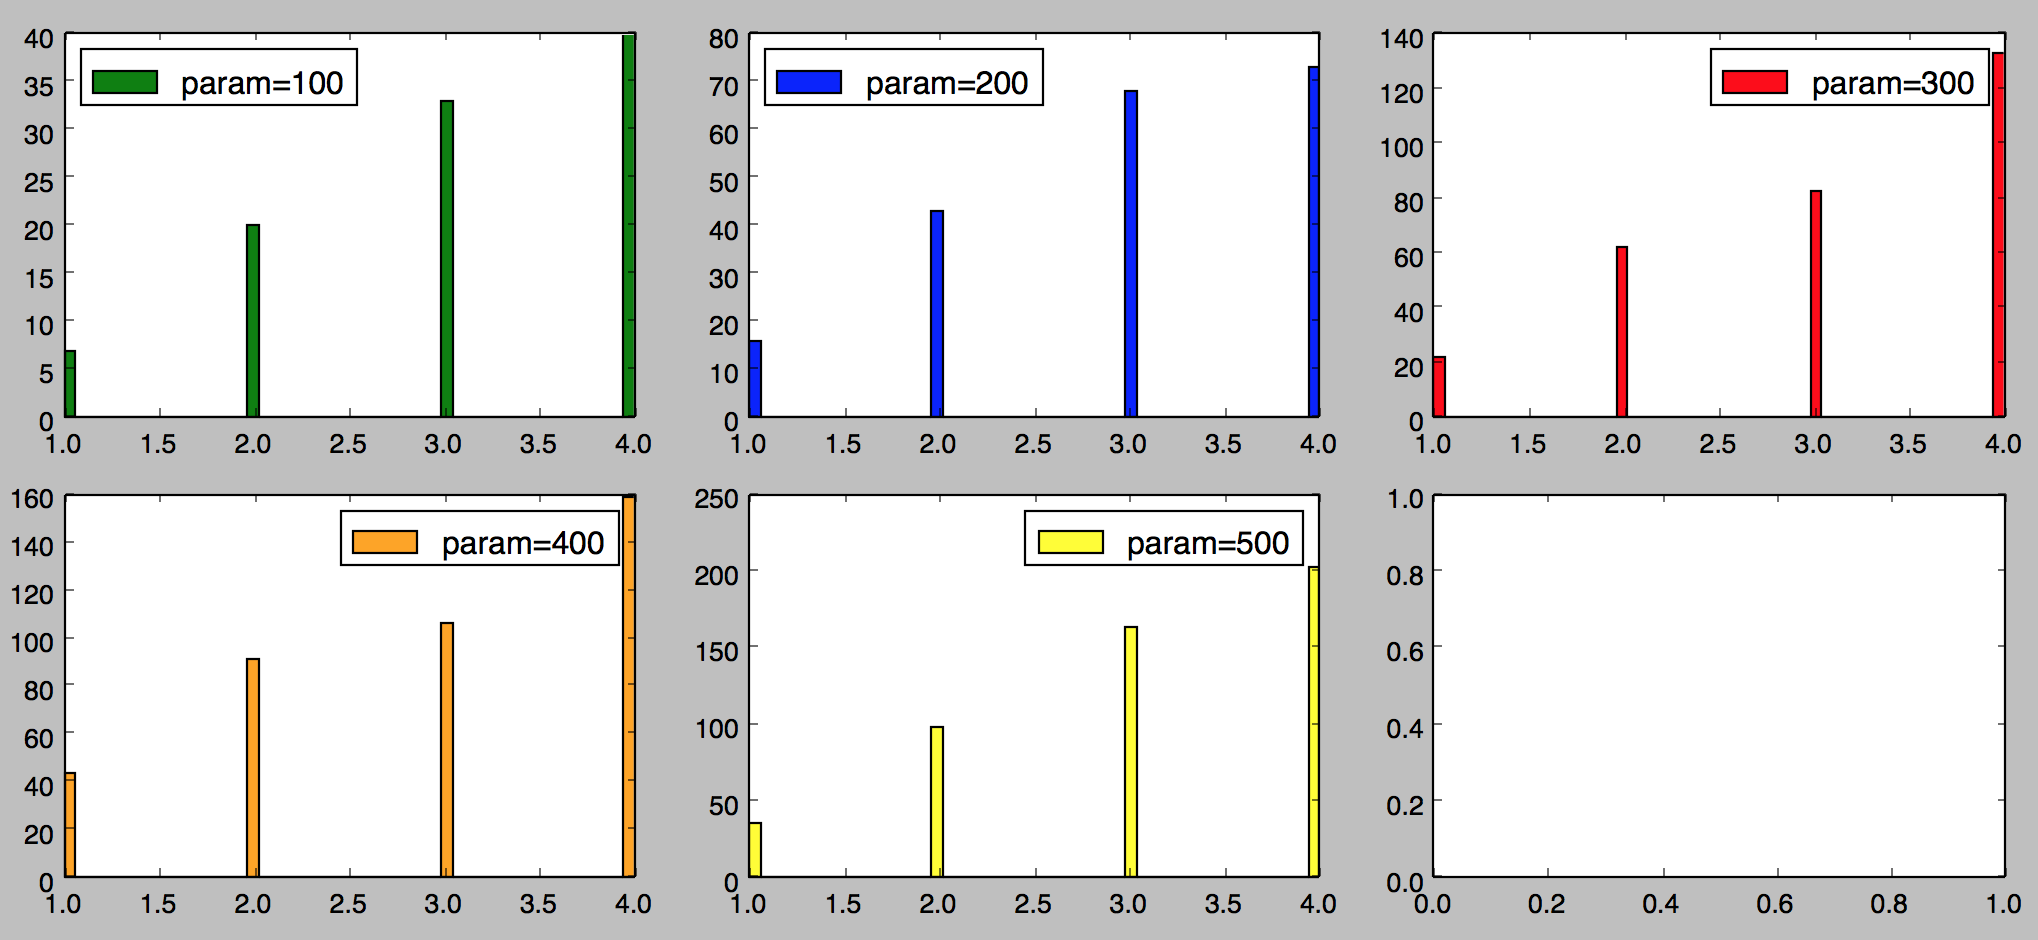
\includegraphics[scale=.4]{images/bootstrap.png}

\subsection*{Part 2}

\begin{enumerate}
\item [2.] On a single plot, show the training and testing error as a function of iteration t.

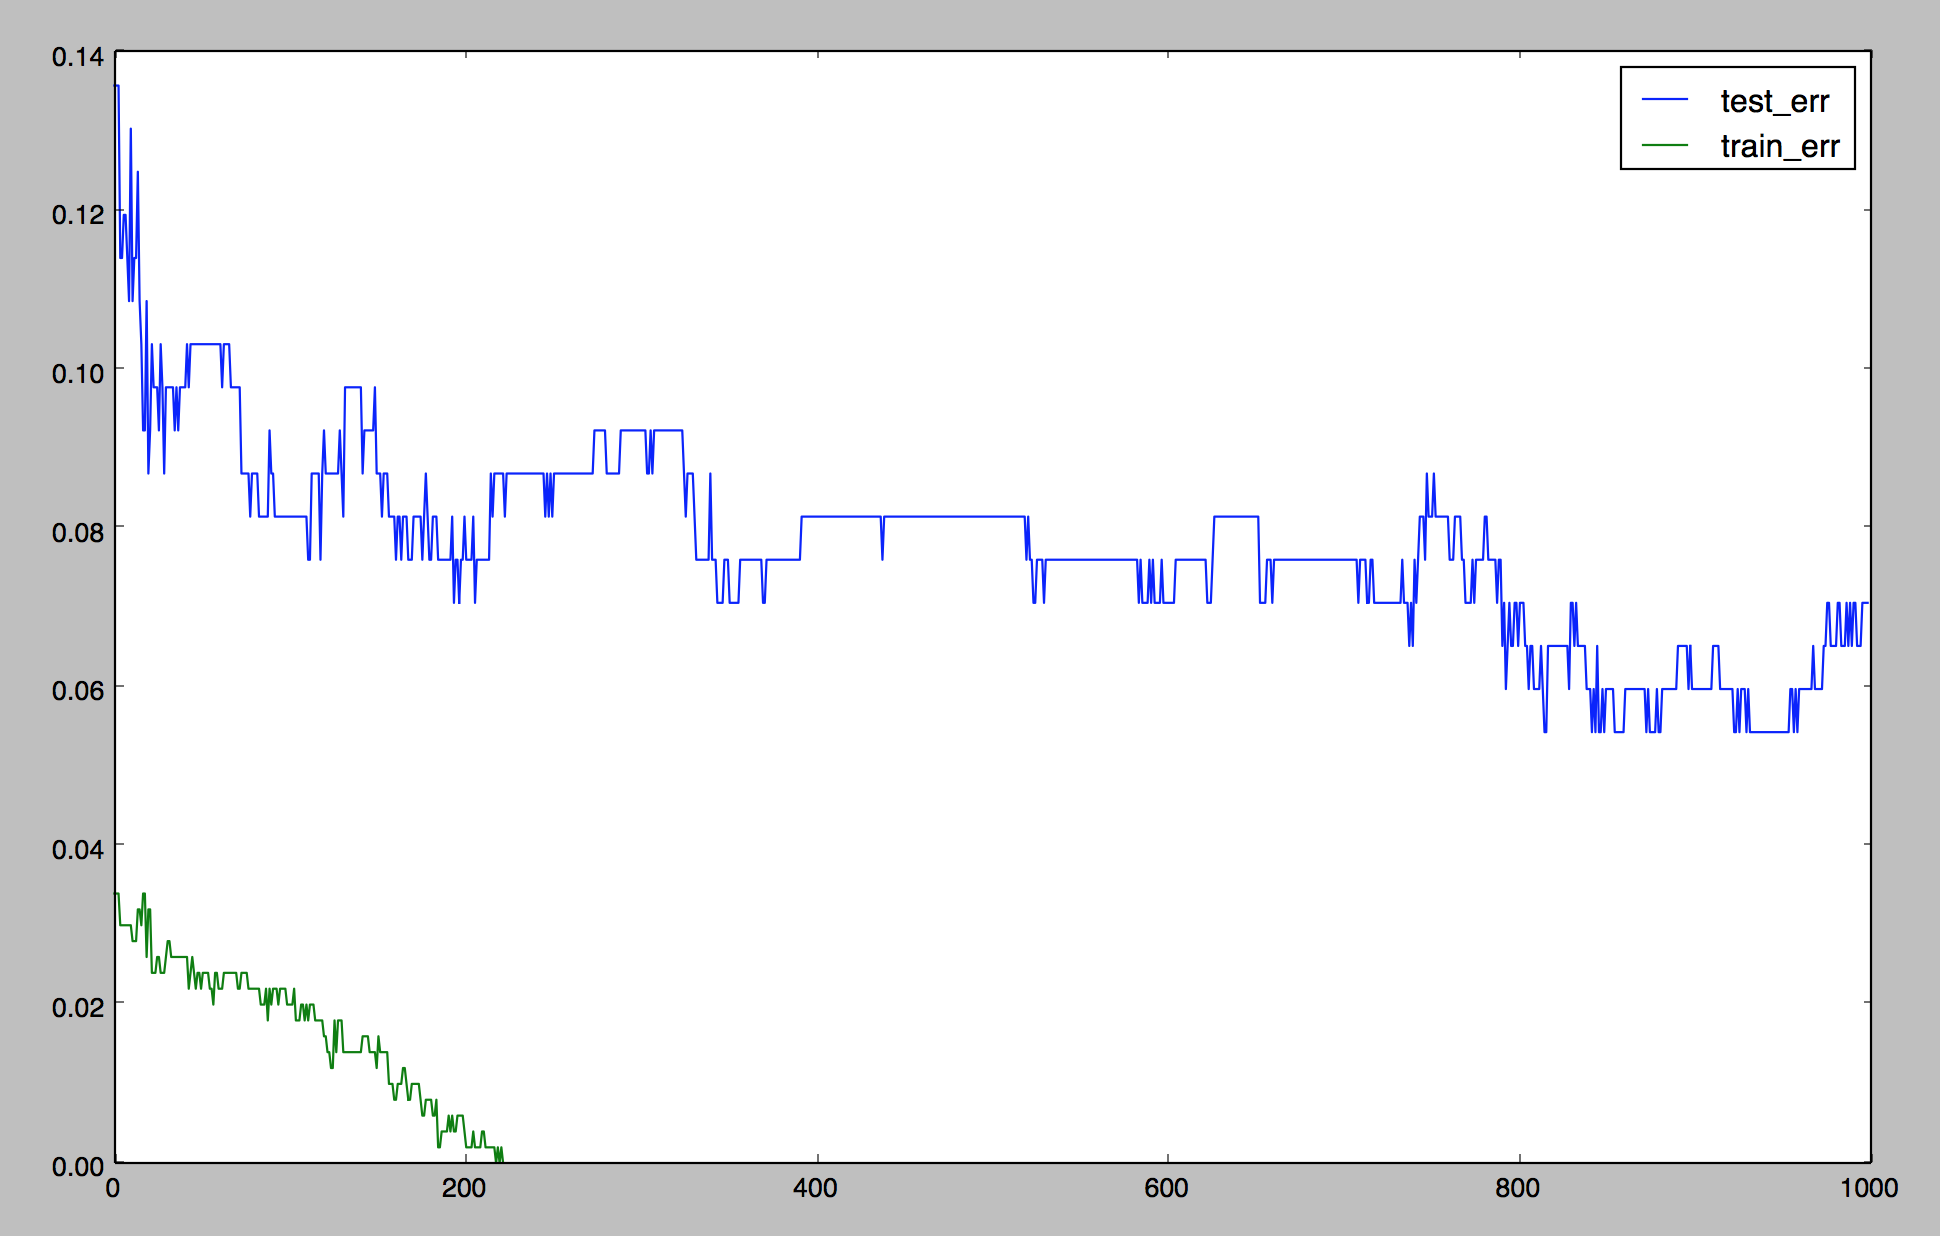
\includegraphics[scale=.4]{images/p2testtrain.png}

\item[3.] Indicate the testing accuracy by learning the Bayes classifier on the training set without boosting.

\begin{table}[!th]
\centering
\begin{tabular}{|c|c|cl}
\hline
& -1 & 1 \\
\hline
-1 & 54 & 27 \\
1 & 2 & 101 \\
\hline
\end{tabular}
\caption{Confusion matrix for Binary Bayes Classifier, accuracy .8423}
\label{ex:table}
\end{table}


\item[4.] Plot $\alpha_t$ and $\epsilon_t$ as a function of $t$.

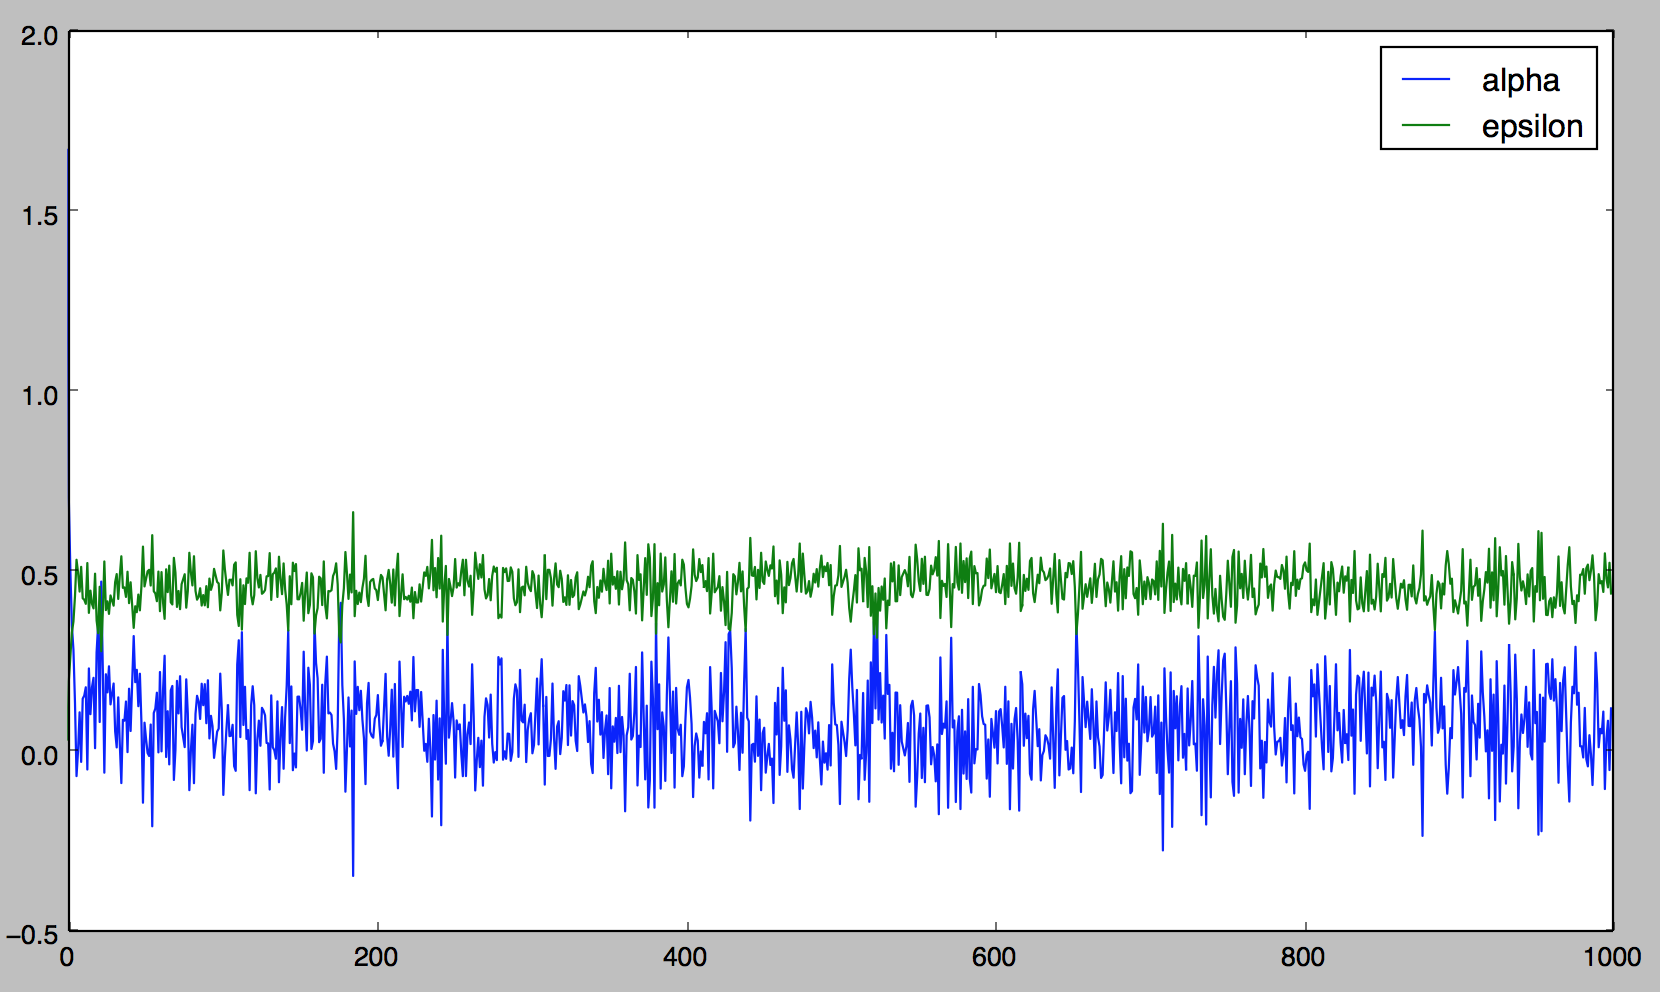
\includegraphics[scale=.5]{images/p2params.png}

\item[5.] Pick 3 data points and plot their corresponding wt(i) as a function of t. Select the points such that there is some variation in these values.

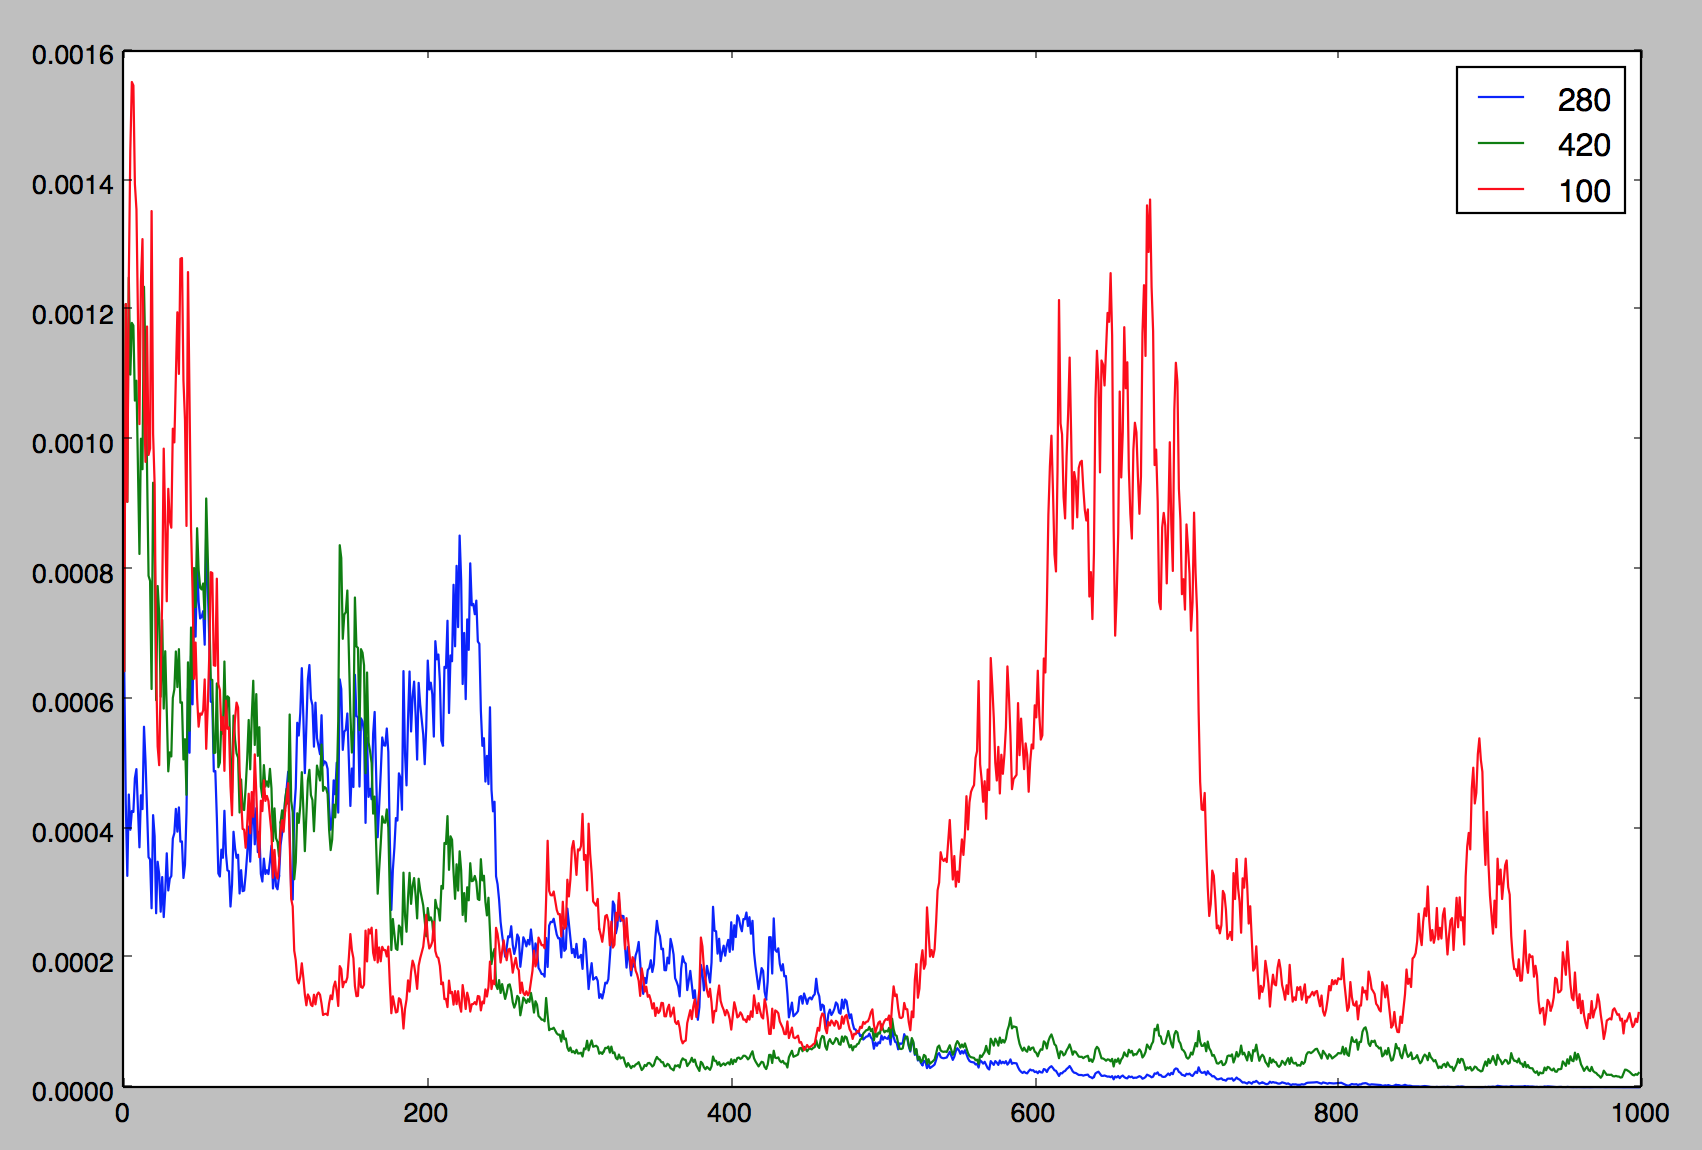
\includegraphics[scale=.5]{images/p2w.png}

\end{enumerate}

\subsection*{Part 3}

\begin{enumerate}
\item [2.] On a single plot, show the training and testing error as a function of iteration t.

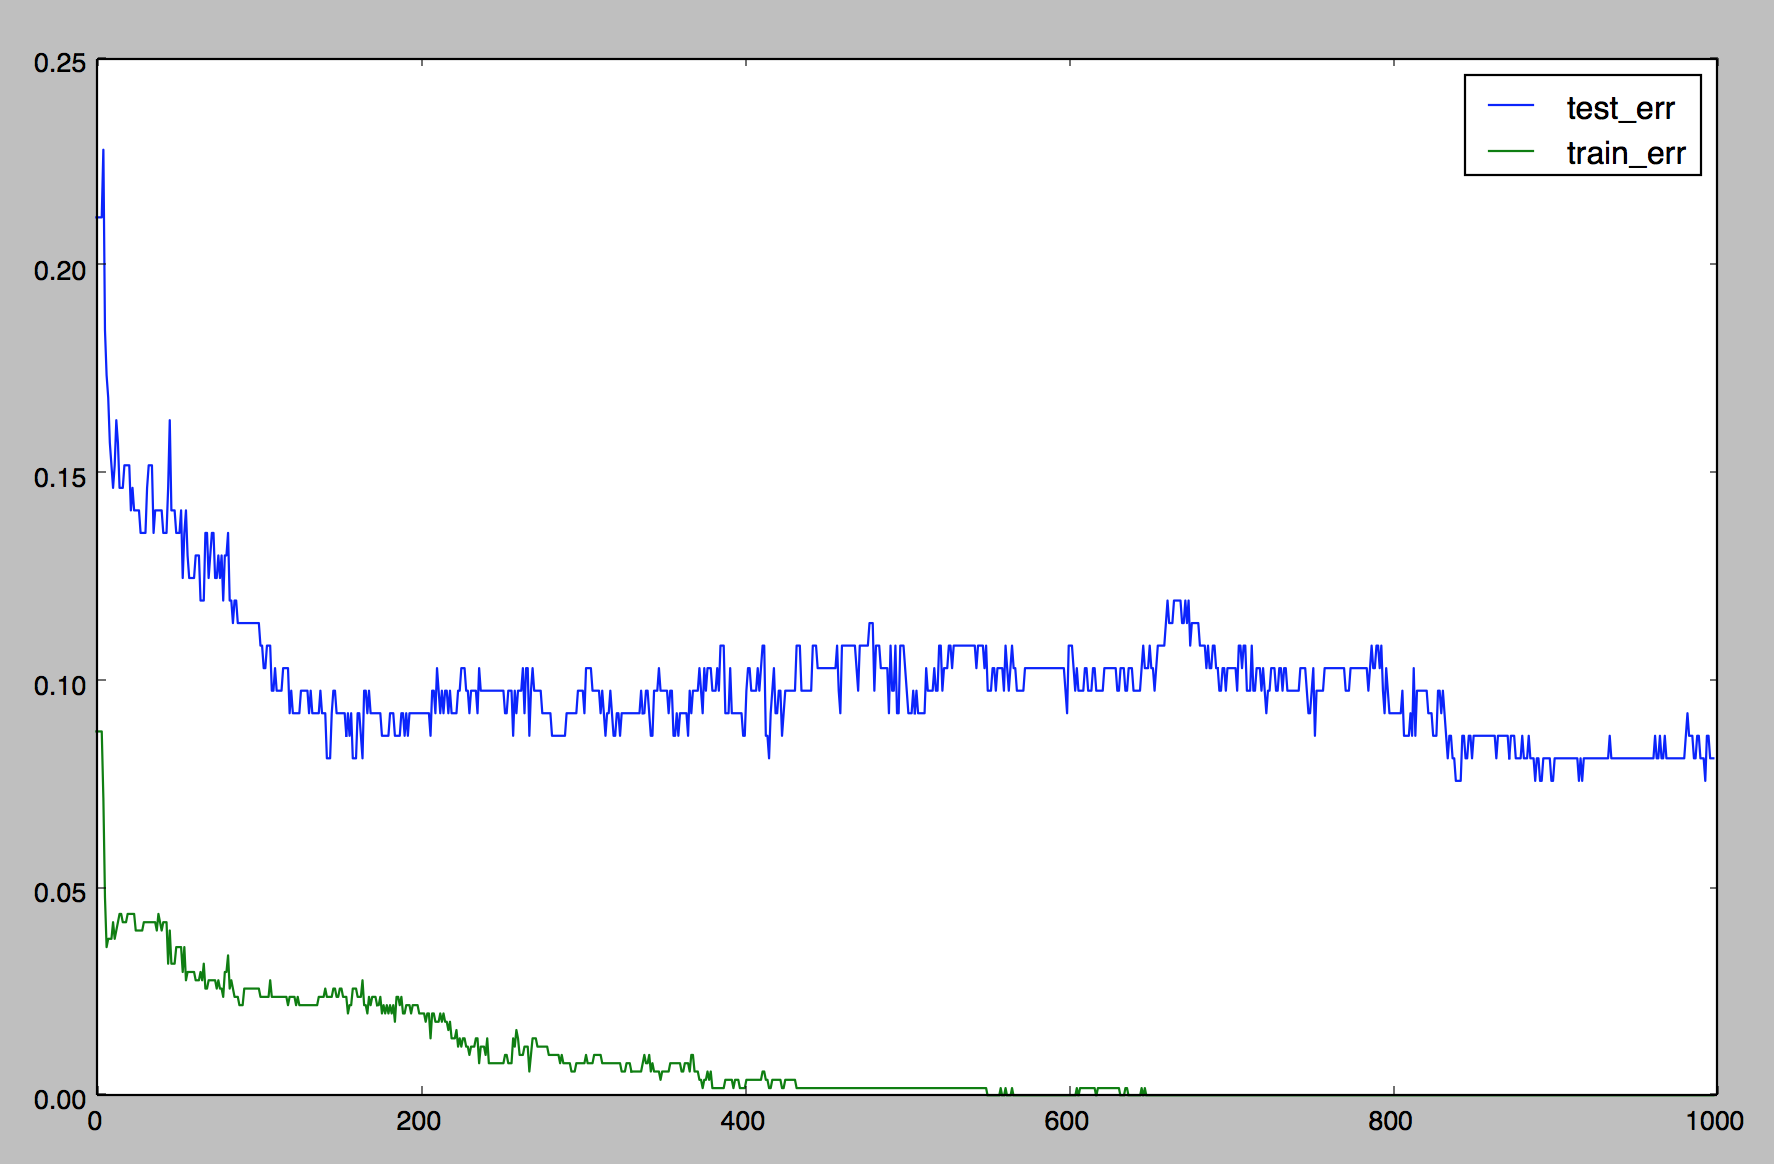
\includegraphics[scale=.5]{images/p3testtrain.png}

\item[3.] Indicate the testing accuracy by learning the logistic regression model on the training set without boosting.

For this problem, I implemented a binary logistic regression classifier.

\item[4.] Plot $\alpha_t$ and $\epsilon_t$ as a function of $t$.

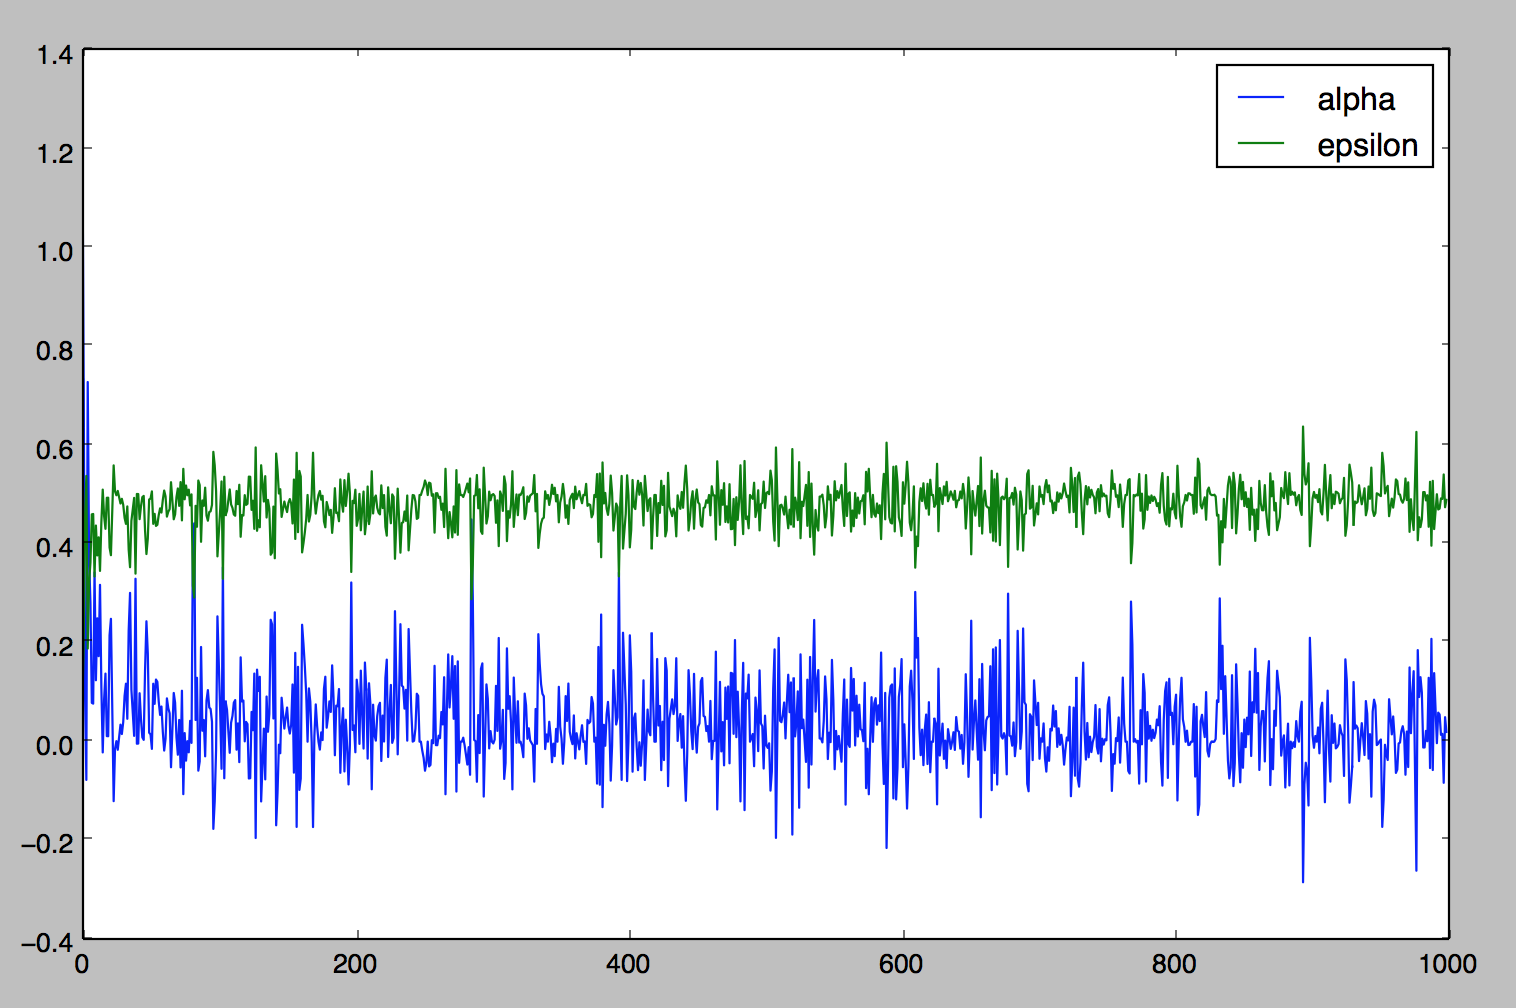
\includegraphics[scale=.5]{images/p3params.png}

\item[5.] Pick 3 data points and plot their corresponding wt(i) as a function of t. Select the points such that there is some variation in these values.

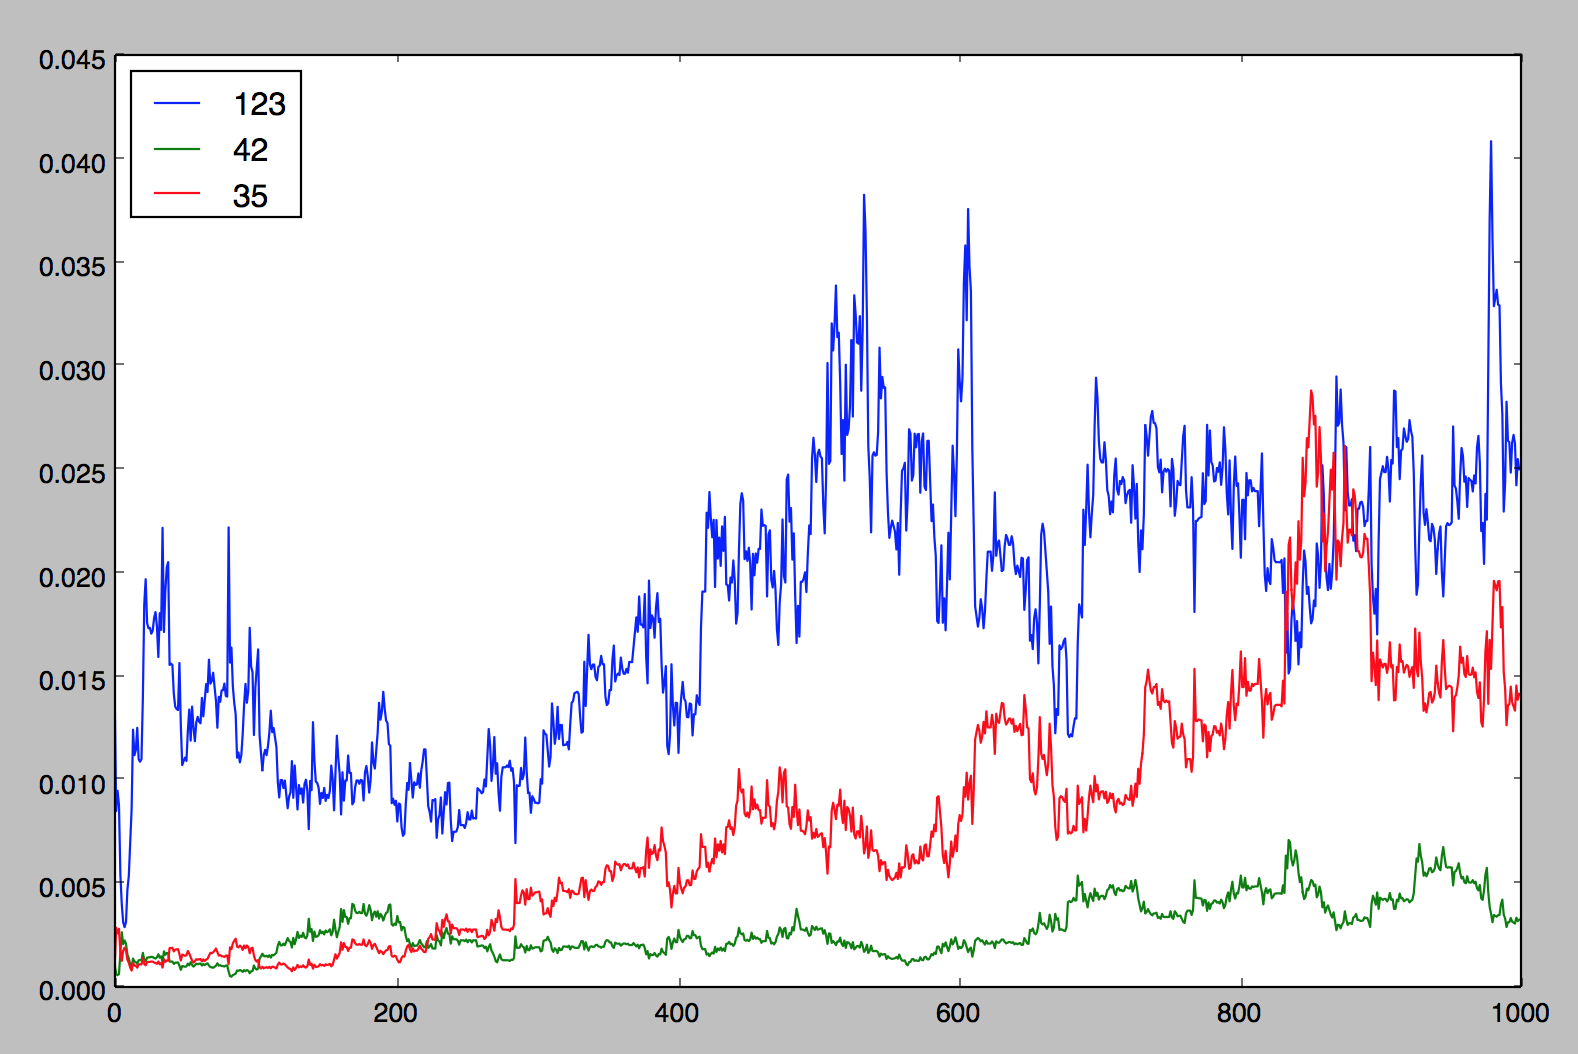
\includegraphics[scale=.5]{images/p3w.png}

\end{enumerate}

\end{document}
